\documentclass{PDS}%


%%%% Packages
\usepackage{graphicx}
\usepackage{multicol,multirow}
\usepackage[fleqn]{amsmath}
\usepackage{amssymb,amsfonts}
\usepackage{amsthm}
\usepackage[figuresright]{rotating}
\usepackage{appendix}
\usepackage[authoryear]{natbib}
\usepackage{ifpdf}
%\usepackage{newtxtext}
%\usepackage{newtxmath}
\usepackage[T1]{fontenc}
\usepackage{textcomp}
\usepackage{xcolor}
\usepackage[colorlinks,allcolors=dscolor,bookmarks=false]{hyperref}




\newtheorem{theorem}{Theorem}[section]
\newtheorem{lemma}[theorem]{Lemma}
\theoremstyle{definition}
\newtheorem{remark}[theorem]{Remark}
\newtheorem{example}[theorem]{Example}
 

\jyear{2025}

\jdoi{https://doi.org/10.1017/pds.2025.xxx}



\begin{document}


\articletype{}%

\title[\color{dscolor}A*-BASED BFO ALGORITHM FOR GLOBAL PATH PLANNING OF USVs]
{An A*-based bacterial foraging optimisation algorithm for~global path planning of unmanned surface vehicles}


\maketitle

\hrule{}
\vspace{35mm}
Leave empty for metadata
\vspace{35mm}
\hrule{}

\section{Introduction}


The development and application of freshwater and marine areas is becoming
increasingly extensive. Owing to the special working requirements of water, most water
operations need to be accomplished by ships. Unmanned surface vehicles (USVs), with the
advantages of flexible controllability, strong autonomy and field operation, have been
widely applied in the civil and military fields, such as maritime cruise ships, emergency rescue
activities, lake patrols and hydrological monitoring \citep{r6,r1,r4,r5,r3,r2}.

In order to guide a USV through a cluttered environment, planning a high-quality and
collision-free path is a critical part during the USV's voyage \citep{r7}. Particularly,
path planning is an important technology in the application of the USV's intelligent
control and an indispensable part of driverless technology, which not only determines the
level of autonomy of the vehicle but also premises the reliability of a mission and the
likelihood of success. Fundamentally, USV path planning is a branch of classical robot
tracing, which mainly concerns two factors: the total path distance and safety
\citep{r8}. In addition, the quality of the generated trajectory, such as smoothness and
continuity, also needs to be taken into account \citep{Smierzchalski1999}.


Path planning
technologies can be generally divided into two groups: the pre-generative approach
(static planning) and the reactive approach (dynamic planning) \citep{r11}.
\citet{ShiBinghua} focused on the smoothness and seaworthiness properties of the path. A
hybrid A* algorithm with motion primitive constraints is proposed to generate an initial
reference path. In order to optimise the path, a number of computational intelligent
algorithms have been applied. A genetic algorithm (GA) is used to determine the optimised
path for a USV under environmental loads in \citet{r15}. The optimised paths are determined
by numerical simulations. An approach of fast path planning based on a Voronoi diagram
and an improved GA has been proposed in \citet{r16}. Furthermore, as a branch of intelligent
algorithms, the swarm intelligence algorithm plays an important role in research on USV
global path planning. \citet{r17} proposed a method for USV global path planning based on
particle swarm optimisation. By using typical obstacle modelling and the ant colony
algorithm (ACO) for global path planning, the USV global path was achieved in \citet{r18}.
\citet{r19} improved the ACO-based grid environment model for USV global path
planning. Meanwhile, some works have been done to combine various intelligent swarm
algorithms for USV global path planning. For example, in \citet{r20}, both GA and ACO
are used to generate an initial pheromone distribution and carry out dynamic integration of
genetic operators, which not only can improve the convergence rate of the algorithm, but also can
solve the problem of precocious and poor global search ability.

The bacterial foraging optimisation (BFO) algorithm is a new bionic algorithm, which has become another hotspot in the field of heuristic
computing. Owing to its advantages, such as parallel searching of the swarm intelligence algorithm
and ease of jumping out from local minima, it has attracted more interest. At present,
BFO has been successfully applied in many fields, such as image processing
(\citealp{r22}; \citealp{r23}; \citealp{r24}), shop scheduling (\citealp{r25}; \citealp{r28}; \citealp{r27}; \citealp{r26}; \citealp{r29}), robotics (\citealp{r32}; \citealp{r31}; \citealp{r33}; \citealp{r30}; \citealp{r34}), etc.

\subsection{Contributions of this paper}

This paper proposes a more efficient grid partition-based hybrid BFO path planning
method, named AS-BFO, by integrating the A* algorithm to enhance the conventional
BFO algorithm, thus solving the issue of the generation of a discontinuous path. The main
contributions of this paper are listed below:
\begin{enumerate}[(3)]
\item[(1)] The bacterial foraging optimisation algorithm is improved and applied in USV
global path planning under the grid environment.

\item[(2)] The cost function of the A* algorithm is integrated into the tumble motion, which
solves the problem of repairing a discontinuous path.

\item[(3)] The relative optimal parameter combination is obtained and it makes the AS-BFO algorithm
run effectively in different working environments.
\end{enumerate}

The rest of the paper is organised as follows. Section~2 describes the basic steps
of the BFO. Section~3 establishes an environmental model and introduces the AS-BFO for
our problem.  At the same time, a repellent signal is
also released to warn other bacteria to keep a safe distance from
itself.  To gather information, corresponding methodologies
(early detection architecture) are used, in which the information gathered through an
intuitive and broad approach is assigned to previously defined
subject areas. The parameter combination simulation and the optimal parameter combination
are obtained, and the sensitivity analysis of AS-BFO parameters is carried out in
Section~4. GA, ACO and AS-BFO are selected for comparison in different experimental
environments. Section~5 concludes this work.

\section{Description of BFO}\label{sec2}

BFO is a global random searching algorithm, whose operation aims to simulate the
physiological behaviour of \textit{Escherichia coli} bacterium in the process of foraging behaviour, the
modelling iteration producing the optimal solution. The cost function of the A* algorithm is integrated into the tumble motion, which
solves the problem of repairing a discontinuous path. The BFO consists of three principal
mechanisms to find the relative optimal solution: chemotaxis, reproduction and
elimination--dispersal, each of which is detailed below (\citealp{r21}; \citealp{r36};
\citealp{r37}; \citealp{r35}).

%%\subsection{Chemotaxis}

In biology, the movement of bacteria is called chemotactic behaviour, and there are two
types of chemotaxis of bacteria: swim and tumble/rotate. The cost function of the A* algorithm is integrated into the tumble motion, which
solves the problem of repairing a discontinuous path. Swimming is the motion of bacteria forwards along the same direction as the last stage; rotation is the bacteria staying in the
same position and rotating itself into a new direction. These two chemotactic operations
guarantee that bacteria search the problem space as well as avoid obstacles in the
searching process. The new position of the bacteria after chemotaxis can be obtained by
\begin{equation}\label{equ:1}
\theta^i(j, k, l)=\theta^i(j+1, k, l)+ C(i)\frac{{\Delta ( i )}}
{{\sqrt {\Delta^\text{T} (i)\Delta ( i )} }},
\end{equation}
where $\theta^i(j, k, l)$ represents the bacterium $i$ in the $j$th chemotaxis, $k$th
reproduction and $l$th elimination--dispersal step, $C(i)$ denotes the size of chemotaxis
during each swim or tumble, and $\Delta (i)$ is the direction vector of the $j$th
chemotactic step. Finally, $\Delta (i)$ is a random direction vector with a range of $[-1, 1]$.
\begin{quote}
Scanning is a validation activity. In the iPeM, validation is understood as a basic
activity of product engineering and is the only activity that generates knowledge.
Scanning is used to detect indicators for the future environment through comprehensive
and undirected screening if no or only very vague information regarding changes in
future development is available. To gather information, corresponding methodologies
(early detection architecture) are used, in which the information gathered through an
intuitive and broad approach is assigned to previously defined subject areas.
\end{quote}
During cell-to-cell communication, when each bacterium moves, it releases attractant
to signal other bacteria to swarm towards it. At the same time, a repellent signal is
also released to warn other bacteria to keep a safe distance from itself. Such a
communication mechanism is also simulated by representing the combined cell-to-cell
attraction and repulsion, which can be expressed by
\begin{align}
J_{cc} (\theta^i(j, k, l) ,\theta(j, k, l)) &= \sum_{i = 1}^S {J_{cc}^i (\theta^i,\theta)}\notag\\
&= \sum_{i = 1}^S {\left[ - d_{\text{attract}} \exp \left( - \omega_{\text{attract}} \sum_{m =
1}^D {(\theta_m - \theta_m^i )^2 } \right)\right]}\notag\\
&\quad +\sum_{i = 1}^S {\left[h_{\text{repellant}} \exp \left( - \omega_{\text{repellant}} \sum_{m =
1}^D {(\theta_m - \theta_m^i )^2 } \right)\right]},
\label{equ:2}
\end{align}
where $J_{cc}^i (\theta^i ,\theta)$ denotes the object function value, which represents a
time-varying objective function, $S$ represents the total number of bacteria, $D$ is the
number of variables to be optimised, and $d_{\text{attract}}$, $\omega_{\text{attract}}$,
$h_{\text{repellant}}$ and $\omega_{\text{repellant}}$ are coefficients representing the
attractive depth, attractive width, repellent height and repellent width, respectively.

\subsection{Reproduction}

After the chemotaxis, the health status of each bacterium is determined by the sum of the
step fitness, i.e. $\sum_{j=1}^{N_c}J(i,j,k,l)$, where $N_c$ is the maximum step in a
chemotaxis process. Based on their health status (fitness values), all bacteria are
sorted.\footnote{In the reproduction step, the half of the bacteria with higher fitness values survive
and the others are eliminated. And then each surviving bacterium splits into two
identical ones. The reproduction process keeps the population of
bacteria constant.}

\subsection{Elimination--dispersal}

In order to avoid the bacteria becoming stuck around the initial positions or local
optima, the elimination--dispersal process is introduced in the BFO. In the
elimination--dispersal process, some bacteria are selected, based on a probability
$P_{ed}$, to be moved to another position within the environment.

\section{AS-BFO for USV global path planning}\label{sec3}

The proposed AS-BFO method is detailed in this section. In particular, given a known map
with a number of obstacles, the proposed algorithm first grid partitions the given map into
an $n \times n$ grid environment. The parameters of AS-BFO are tightly coupled. The selection of the parameters
directly affects the performance of the algorithm. Then, the conventional BFO algorithm is applied to
find the optimal path. During the chemotaxis operations of the BFO, each step will be
monitored to check whether  or not  the tumbled node is continuous with the previous node as well
as the following node. The parameters of AS-BFO are tightly coupled. The selection of the parameters
directly affects the performance of the algorithm. If any discontinuous path is identified, the A*
algorithm is employed to repair the discontinuous part. This process will be applied
until an optimal solution is found. The final optimal solution will be the best path for the
given map. The flowchart of the proposed method is shown in Figure~\ref{fig:1}, and
the key components are detailed below.
\begin{figure}[h!]
\centering{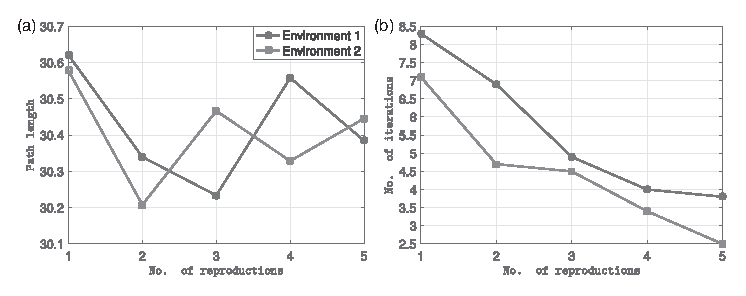
\includegraphics{PDS_fig1}}
\caption{Flowchart of AS-BFO}
\label{fig:1}
\end{figure}
 
The grid method is an effective modelling method. The method is easy to construct, modify
and simulate the geographical environment. The grid map not only can simulate relatively
accurate environmental information for the USV, but also can provide simulation environments of
different sizes and complexity for algorithm experiments. This provides a good basis for
analysing the performance of the algorithm.\footnote{The electronic chart is a digital chart that is a
type of map model for USV global path planning.} Electronic charts can provide map
information for USVs, but such maps are less flexible than grid maps. The parameters of AS-BFO are tightly coupled. These two chemotactic operations
guarantee that bacteria search the problem space as well as avoid obstacles in the
searching process. The selection of the parameters
directly affects the performance of the algorithm. A cellular grid map
is also applied to the study of global path planning. However, in cellular grid maps, the
minimum steering angle can only reach 60$^{\circ}$, so the grid map has an advantage in
steering angle. USVs usually work in vast stretches of water.


The work environment can be considered
as a two-dimensional space with static obstacles. Therefore, the working environment of a
USV can be gridded. In the general analysis, if obstacles occupy less than one grid, it
will be considered as one whole grid (\citealp{r33}). Thus, it will establish a
one-to-one correspondence between the grid number and the
two-dimensional coordinates. These two chemotactic operations
guarantee that bacteria search the problem space as well as avoid obstacles in the
searching process. The data structure of the algorithm is a nine-square graph centred on the current node,
with a total of eight adjacent nodes. The following node must be chosen from these eight
neighbours. In the $n\times n$ grid environment.
\begin{itemize}
\item The bacterial foraging optimisation algorithm is improved and applied in USV
global path planning under the grid environment.

\item The cost function of the A* algorithm is integrated into the tumble motion, which
solves the problem of repairing a discontinuous path.

\item The relative optimal parameter combination is obtained and it makes the AS-BFO algorithm
run effectively in different working environments.
\end{itemize}
where mod(.) is the remainder operation and $\text{ceil}(\cdot)$ rounds an element to
the nearest integer towards positive infinity. As mentioned above, the goal of path
planning is to find an ordered grid with the shortest distance among feasible ordered
grids.

\subsection{Coding method}

The population described in this paper consists of a limited number of bacteria. Each
bacterium is connected by a series of nodes. One bacterium represents a feasible path. It
should be noted that, owing to the randomly generated paths being composed of different
numbers of nodes, the lengths of the paths are not uniform. Therefore, variable length
bacteria are used to represent individuals. Figure~\ref{fig:2} shows a path and its
corresponding bacterium.

\begin{figure}[h!]
\centering{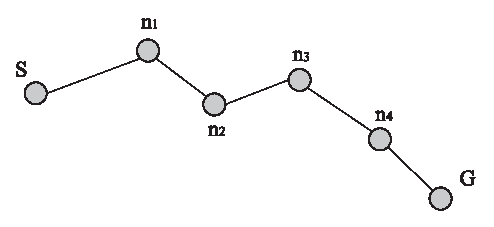
\includegraphics{PDS_fig2}}
\caption{A feasible path}
\label{fig:2}
\end{figure}


%\subsection{Three operators of AS-BFO}
%\subsubsection{Chemotaxis}

This paper defines the chemotaxis operation of BFO in the grid environment. Chemotaxis in
traditional BFO means that any nodes will tumble and swim in any direction. However, some
tumbling motions can result in discontinuous paths in the grid environment. Therefore, AS-BFO
improves the chemotaxis operator. Firstly, it judges whether the tumbled nodes are
continuous with the previous and the following nodes. Then, the discontinuous paths are
repaired using the A* algorithm. 
\begin{quote}
Monitoring is a targeted search for in-depth information on the development of
previously identified indicators for the future environment that are potentially relevant
for the company's own process and system development. By systematic and continuous
observation of selected indicators during development, monitoring enables the early,
cross-generational recognition of changes in future development and thus supports the
definition and introduction of suitable actions.
\end{quote}
Currently, monitoring is mainly used to update company strategies. However, it is useful to make it
available for the cross-generational product development approach to make the process agile and
adaptive. Boundary conditions, objectives and requirements are often uncertain and vague in the early
stages. The closer the product comes to market launch, the clearer but also more restrictive these
become. Monitoring should be used to identify and take account of changes as early as possible. This
should involve a two-way networking of the information flow with feedback between the boundary
conditions and premises derived from the foresight and the solutions being developed for the various
product generations to check their validity. This requires the definition of indicators that enable targeted
and comprehensible monitoring of individual aspects for all generations in different stages of a product.
These are defined within the activity scanning and could be, for example, changed trends or adapted
laws that significantly influence a specific product characteristic. If a change with an impact on the
underlying environment, technology or product scenarios is identified at a certain time, it is necessary
to assess whether this has a relevant impact on the properties and design of the product generations
currently under development. If this is the case, its extent must be assessed and the various options for
action must be weighed up for a decision. A decision could also be to launch the next generation as
planned as changes would take too much time to implement but consider the new information to adapt
further generations that are already in development.
When the chemotaxis operator is performed, the following situations are possible.
Firstly, after the node is tumbled, the tumbled node is continuous with its previous and
following nodes, as shown in Figure~\ref{fig:3}. These can be trends, prognoses or laws, for example, which
must be linked to the product properties. Trend radars, the development of certain competitors' products,
technological developments and social debates on specific topics are possible points of reference. The
initial search is undirected but may be based on the underlying scenarios. In strategic foresight, there
exist approaches and methods If $n_2$ is a tumble node, it can be
randomly tumbled to the adjacent free grids. Taking Figure~\ref{fig:3} as an
\hbox{example,} $n_2$ tumbles to $n'_2$. Then, according to Equation~(4), it is judged
whether $n_1$ and $n'_2$, $n'_2$ and $n_3$ are, respectively, continuous. If $\Delta=1$, then
$n_1$ and $n'_2$, $n'_2$ and $n_3$ are continuous; otherwise, they are not: 
\begin{figure}[h!]
\centering{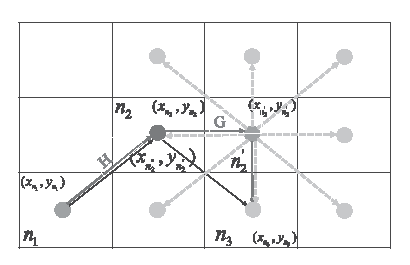
\includegraphics{PDS_fig3}}
\caption{Schematic diagram of continuous nodes}
\label{fig:3}
\end{figure}

Here
$(x_{tumbled}, y_{tumbled})$ are the horizontal and vertical coordinates of the tumbled
node ($n'_2$) and $(x, y)$ are the horizontal and vertical coordinates of the previous or
the following node $(n_1, n_3)$. The path after the tumble motion is marked by the red
line.

Secondly, it is discontinuous with the previous or the following node, when the node is
tumbled. As shown in Figure~\ref{fig:4}(a), $n_2$ is used as the tumble node. So $n_2$ is
tumbled to $n'_2$, and then it is judged whether $n_1$ and $n'_2$, $n'_2$ and $n_3$ are,
respectively, continuous. It can be observed that $n'_2$ and $n_3$ are continuous;
however, $n'_2$ and $n_1$ are not continuous. At this time, the evaluation function of
the A* algorithm is applied to the tumble motion, and the problem of repairing the
discontinuous path has been solved. Figure~\ref{fig:4}(b) shows that there are many
repaired nodes around $n'_2(x, y)$, and the yellow nodes are repaired nodes.

\begin{figure}[h!]
\centering{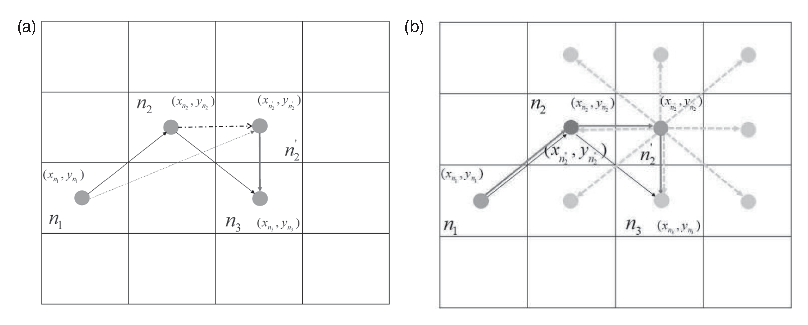
\includegraphics{PDS_fig4}}
\caption{Schematic diagram of discontinuous nodes. (a) Intermittent path, (b) Patching path}
\label{fig:4}
\end{figure}

A repaired node will be selected depending on Equations (5)--(7):
\begin{align}
&F_{\min } = G + H, \label{equ:5}\\
&G = \sqrt {(x_{\text{tumbled}}' - x_{\text{tumbled}}'' )^2 + (y_{\text{tumbled}}' - y_{\text{tumbled}}'' )^2 }, \label{equ:6}\\
&H = \sqrt {(x - x_{\text{tumbled}}'' )^2 + (y - y_{\text{tumbled}}'' )^2}. \label{equ:7}
\end{align}
Here $(x, y)$ represents the coordinates of the previous node, $(x'_{\text{tumbled}}, y'_{\text{tumbled}})$ denotes the coordinates of a node after it has been tumbled, and
$(x''_{\text{tumbled}}, y''_{\text{tumbled}})$ indicates the coordinates of the repair
nodes. As shown in Figure~\ref{fig:4}(b), we use $(x''_{n_2}, y''_{n_2})$ as the
coordinates of the repaired node. When the discontinuous path is repaired, it is
represented by the red line. Although the path increases slightly, this method solves the
problem that the path is discontinuous after the node is tumbled.

This paper introduces a novel methodology for analyzing the spatial distribution and co-presence of
objects within home interiors utilizing graphs. This approach entails constructing a graph where nodes
represent individual objects, such as furniture or decor, and edges denote these objects' co-presence or
relational adjacency within a given space, such as a specific function of an entire home. The weight of
each edge corresponds to the frequency or significance of the co-presence of the connected objects. This
method facilitates an analysis of object-to-object relationships and their centrality within the domestic
environment. A quantified domestic activities trend is enabled where traditionally invested based on the
attributes of the physical environment, such as size, connectivity, and layout of the homes. In this graph,
unique object pairs are extracted to ensure no repetition of objects
within a single graph representation. 



Finally, the tumbled node is discontinuous with the previous node and the following node after
the node is tumbled. Then, the repaired point can be found by
Equations~(5)--(7) so that the path is continuous. Note that we need
to use the evaluation function of the A* algorithm twice in this condition.
The method to deal with discontinuity with the previous and the following nodes is the
same as the above method. Therefore, an effective method to repair discontinuous paths is
proposed, which ensures that each tumble can be performed efficiently.


\subsubsection{Reproduction}

When the chemotaxis operation is completed, the path length represented by each bacterium
is sorted. The half of the bacteria with longer paths are eliminated, and the half of the bacteria
with shorter paths are reproduced. Thus, bacteria number is kept unchanged.

\subsubsection{Elimination--dispersal}

When the reproduction operation is completed, a random probability $P_r$ is generated and
compared with the fixed migration probability $P_{ed}$. If $P_r$ < $P_{ed}$, the
bacterium is dispersed. This operation can reduce the possibility of bacteria falling
into a local optimal solution. It can also be a good solution for maintaining diversity.

\subsection{Algorithm description}

In this algorithm, the path optimisation problem is encoded. One feasible path
represents one bacterium. The initial population is usually randomly generated without
infeasible paths, which can reduce the blindness of initial population generation. Among
the three main operators in the algorithm, the chemotaxis operator can improve the local
search accuracy of bacteria, the reproduction operator can increase the convergence
performance of bacteria, and the elimination--dispersal operator can increase the diversity of
solutions. The parameters of AS-BFO are tightly coupled. The selection of the parameters
directly affects the performance of the algorithm. At present, there is no perfect
theoretical basis to determine the optimal combination parameters. The traditional method
is repeated trials to obtain the relative optimal combination of parameters.


\section{Analysis of results}\label{sec4}

It is very important for the application of AS-BFO in practical problems to study the
parameters of population size, chemotaxis number, replications number and
elimination--dispersal number. However, the setting of the parameters mainly depends on
the statistical data and simulation experiment. This paper studies the path planning in
two different environments, in which the islands represent the obstacles.

\subsection{Experiment 1}

Different parameter settings may lead to different performances. In this experiment,
different parameters are applied in the proposed method, in order to compare the
performances generated by different parameter settings.

\subsubsection{Population number}

In this experiment, the chemotaxis number $N_c=5$, reproduction number $N_{re}=2$ and
elimination--dispersal number $N_{ed}=2$ are fixed, and the population number $P$ is selected
to be 10, 20, 30, 40, 50, 60, 70 and 80, respectively. The results show that the greater the number of bacteria, the faster the convergence rate.

\subsubsection{Chemotaxis number}

The chemotaxis operator is an important operator of AS-BFO, and the chemotaxis number
directly affects the local optimisation ability of the algorithm. In this simulation
experiment, $P=50$, $N_{re}=2$ and $N_{ed} =2$ are fixed, and the chemotaxis number is set to $N_c
=1$, 2, 3, 4, 5, 6, 7 and 8. For environment
1, when $N_c =7$, the path is the shortest. When $N_c =8$, the number of iterations is
the least. For environment 2, when $N_c =8$, the path is the shortest. When $N_c =6$, the
number of iterations is the least.


\subsubsection{Reproduction number}

The reproduction operator reduces population diversity and increases the convergence rate of
the algorithm. In the simulation experiment, $P=50$, $N_c =5$ and $N_{ed}=2$ are fixed, and the
reproduction number is set to $N_{re}=1$, 2, 3, 4 and 5. For environment 1, when $N_{re}=5$, the path is the shortest. When
$N_{re}=4$, the number of iterations is the least. For environment 2, when $N_{re}=2$, the
path is the shortest. When $N_{re}=5$, the number of iterations is the least.

\subsubsection{Elimination--dispersal number}

The elimination--dispersal operator is designed to improve global optimisation and
maintain the diversity of solutions. As the outermost nesting of the algorithm, the
elimination--dispersal number directly affects the algorithm running time. In the
simulation experiment, $P=50$, $N_c=5$ and $N_{re}=2$ are fixed, and reproduction number varies as $N_{ed}=1$,
2, 3, 4 and 5. For environment 1, when
$N_{ed}=3$, the path is the shortest. When $N_{ed}=5$, the number of iterations is the
least. For environment 2, when $N_{ed}=4$, the path is the shortest. When $N_{ed}=4$, the
number of iterations is the least.
There are four uncertain parameters, population number $P$, chemotaxis number $N_c$,
reproduction number $N_{re}$ and elimination--dispersal number $N_{ed}$, involved
in the proposed model. Table~\ref{table:morrisSamples} shows the sampling ranges of each
parameter during the sampling processes of the Morris method.
\begin{table}[!h]
\centering
\caption{Sampling range of each parameter\label{table:morrisSamples}}
\begin{tabular*}{20pc}{@{\extracolsep\fill}lc@{\extracolsep\fill}}
\toprule
 Parameter & Range \\
\midrule
 Population number ($P$) & $P\sim(10,100)$ \\
 Chemotaxis number ($N_c$) & $N_c\sim(2,12)$ \\
 Reproduction number ($N_{re}$) & $N_{re}\sim(1,8)$ \\
 Elimination--dispersal number ($N_{ed}$) & $N_{ed}\sim(1,10)$ \\
\botrule
\end{tabular*}
\end{table}
As demonstrated above, different values of parameters lead to completely different
results. The most influential parameters are identified by sensitivity analysis (SA), as
well as to understand their impact on the model output. For this reason, the Morris
method \citep{cadero2018global} is applied to develop the parameter sensitivity analysis.
Briefly, the Morris method involves the generation of uncertain parameter samples via a
trajectory-based sampling process. The method calculates and evaluates the standard
deviation $\sigma_i$ of the elementary effects $\mu_i$, where $i$ is the $i${th} date
sample, over $r$ repetitions to assess the factors' importance. A high value of $\mu_i$
indicates a high linear effect for a given factor, while a high value of $\sigma_i$
represents either nonlinear or non-additive factor behaviour. The importance of input
factors of the model can often be assessed by plotting the factors ($\mu^{*},\sigma$),
where $\mu^*$ is the mean of $\mu_i$ in  two-dimensional space. The factors closest to
the origin are less influential.

Preliminary conversations with stakeholders in Trondheim highlighted that the context of work migrants
in the building and construction industry is not completely understood or clearly communicated, which
makes it difficult to propose new strategies to combat modern slavery and inadequate work and housing
conditions. The comprehensive representation of stakeholders was unclear, and there is no regional
policy for providing inclusive housing for work migrants, even though the city has established inclusive
housing strategies specifically for refugees. Our aspiration was that design could help illustrate the full
picture, identify new areas of intervention, and see new possible connections that can propose a new
future of how to regard housing for work migrants in the city.


\subsection{Parameter sensitivity analysis}

 In this experiment, the
Morris method runs a model with five factors along four trajectories, and a total of 20 samples have
been extracted, as listed in Table~\ref{table:samples}. Each generated data sample is
applied as the input to the proposed method 10 times to get an average optimal path
length. According to the Morris method, the
corresponding standard deviation $\sigma$ and its elementary effects $\mu$ for each
trajectory can be calculated, shows the sensitivity of each parameter in the environmental map of different sizes. In
addition, the ($\mu^*,\sigma$) is also plotted in a two-dimensional plot, for parameter importance analysis. It is clear that parameter 3
($N_{re}$) and parameter 4 ($N_{ed}$) are away from the origin, which indicates that
those parameters are the most important.
Within several stages of the framework, the interpretation of
multiple data streams in mixed formats is pivotal. The effectiveness of this will rely on the ability to
interpret the data streams, which will rely on the expertise at hand, the computational resource available,
data storage facilities, the data stream quality, applicability, and suitability to the problem amongst other
factors. This also plays into the balancing of a mixed-method approach. As illustrated in Section 4, the
quantification of human preferences could potentially remove the nuances, and the incorporation of
qualitative feedback in a computational space is challenging.

\begin{table}[h]
\centering
\caption{Extracted samples\label{table:samples}}
\begin{tabular}{@{\extracolsep\fill}lcccc@{\extracolsep\fill}}
\toprule
Factor & \multicolumn{1}{p{6pc}}{\centering Trajectory 1 ($P,N_c,N_{re},N_{ed}$)}
& \multicolumn{1}{p{6pc}}{\centering Trajectory 2 ($P,N_c,N_{re},N_{ed}$)}
& \multicolumn{1}{p{6pc}}{\centering Trajectory 3 ($P,N_c,N_{re},N_{ed}$)}
& \multicolumn{1}{p{6pc}}{\centering Trajectory 4 ($P,N_c,N_{re},N_{ed}$)} \\
\midrule
 1 & (63,2,3,7) & (100,2,8,3) & (10,5,6,10) & (30,2,1,10) \\
 2 & (63,5,3,7) & (100,9,8,3) & (10,2,6,10) & (30,5,1,10) \\
 3 & (30,5,3,7) & (100,9,8,7) & (10,2,6,1) & (63,5,1,10) \\
 4 & (30,5,3,1) & (10,9,8,7) & (30,2,6,1) & (63,5,6,10) \\
 5 & (30,5,1,1) & (10,9,6,7) & (30,2,8,1) & (63,5,6,3) \\
\botrule
\end{tabular}
\end{table}

The performance of the proposed method is evaluated and validated in this section. Generally
speaking, GA and ACO are adopted to against the proposed approach. Likewise, we first
obtain the relative optimal parameters of ACO and GA through repeated experiments in the
S3 environment, and then apply the parameters to other environments. In order to
evaluate the performance of each method under different environments, the simulated
environments, are grid partitioned into five different
size, denoted as: S1, $10\times 10$; S2, $15\times 15$; S3, $20\times 20$; S4, $25\times 25$; and S5, $30\times 30$. Each size is considered as an individual scenario. In each
environment, the ratio of the obstacle area to the entire map area is approximately
equal. The experimental results of three approaches under five different sizes are listed shows the relative optimal paths of the
two environments in the five size maps.

From Table~1, we can see that the AS-BFO has a better average path
length using a very small iteration number. Moreover, the maximum path length obtained by
AS-BFO is less than ACO and GA in the 20 repeated experiments. In S1, S2 and S3,
AS-BFO's AIN has a great advantage. However, the advantages in MaxPL, MinPL and APL are
not obvious. In S4, the advantage of AS-BFO's AIN is still obvious. It is worth noting
that AS-BFO's MaxPL is 24{.}39 (32{.}04) smaller than ACO and 6{.}83 (5{.}07) smaller than GA.
AS-BFO's MinPL is 6 (14{.}49) smaller than ACO and 1{.}76 (0{.}59) smaller than GA. In S5, the
advantages of MinPL's AIN are equally obvious. AS-BFO's MaxPL is 76{.}67 (53{.}01) smaller
than ACO and 17{.}66 (12) smaller than GA. The MinPL of AS-BFO is 40{.}39 (57{.}93) smaller
than ACO and 3{.}76 (2{.}58) smaller than GA. Analysis shows that the larger the map size $L$,
the greater the advantage of AS-BFO. Therefore, AS-BFO is superior to GA and ACO in
searching efficiency and obtaining an optimal solution.

\section{Conclusions}\label{sec5}

This paper proposes a more efficient path planning method based on the AS-BFO algorithm. The
effects of bacteria number, chemotaxis number, reproduction number and
elimination--dispersal number on the global path planning are analysed. Through
experimental analysis, bacteria number is inversely proportional to the path length. The
greater the chemotaxis number, the stronger is the local optimisation ability of the algorithm.
Correspondingly, the path length and iteration number will decrease. However, the greater the
reproduction number, the smaller the diversity of the population and the faster the convergence
of the algorithm. The experiments indicate that the increase of elimination--dispersal
number will decrease both the path length and iteration number within  a certain range. It
can be found from the comparison of algorithms that AS-BFO performs better than
comparative algorithms in terms of average iteration number, average path,
maximum path and minimum path. A parameter sensitivity analysis shows that the effects
between the various parameters and the effect of each parameter on the output are
different in different environmental maps.

\begin{Backmatter}


\section*{\color{dscolor}Acknowledgments}
We would like to express our sincere thanks to Wuhan University of Technology (WHUT) for supporting our work.



\begin{thebibliography}{}

\bibitem[Cadero et al.(2018)]{cadero2018global}
{Cad\'ero, A., Aubry, A., Brun, F.,   Dourmad, J. Y., Sala\'l\'zn, Y.  and Garcia-Launay, F.} (2018).
Global sensitivity analysis of a pig fattening unit model simulating technico-economic performance and environmental impacts.
\textit{Agricultural Systems}, {165}, 221--229.

\bibitem[Cao(2015)]{r16}
{Cao, L.} (2015). Improved Genetic Algorithm for Fast Path Planning of USV.
\textit{International Symposium on Multispectral Image Processing and Pattern Recognition (MIPPR2015)}, 9815, 981529.

\bibitem[Cheng et al.(2015)]{r27}
{Cheng, Z., Tong, Y., Shen L. and Ming, L. I.} (2015). Improved bacteria foraging optimisation algorithm for solving flexible job-shop scheduling problem.
\textit{Journal of Computer Applications}, 63--67.

\bibitem[Frantisek et al.(2014)]{r34}
{Frantisek, D., Babinec, A., Kajan, M., Florek, M. and Fico T.} (2014).
Path planning with modified A star algorithm for a mobile robot. \textit{Procedia Engineering}, {96}, 59--69.

\bibitem[Hossain and Ferdous(2015)]{r37}
{Hossain, M. A. and Ferdous, I.} (2015).
Autonomous robot path planning in dynamic environment using a new optimization technique inspired by bacterial foraging technique.
\textit{Robotics and Autonomous Systems}, {64}, 137--141.

\bibitem[Hu et al.(2015)]{r20}
{Hu, Y., Li, D. and Ding Y.} (2015). A Path Planning Algorithm Based on Genetic and Ant Colony Dynamic Integration.
\textit{IEEE Intelligent Control and Automation}, 4881--4886.

\bibitem[Jati et al.(2012)]{r32}
{Jati, A., Singh, G. and Rakshit, P.} (2012). A Hybridisation of Improved Harmony Search and Bacterial Foraging for Multi-Robot Motion Planning.
\textit{IEEE Evolutionary Computation}, 1--8.

\bibitem[Kim et al.(2017)]{r15}
{Kim, H., Kim, S. H., Jeon, M., Kim, J. H., Song, S. and Paik, K. J.} (2017).
A study on path optimization method of an unmanned surface vehicle under environmental loads using genetic algorithm.
\textit{Ocean Engineering}, {142}, 616--624.

\bibitem[Kushwaha et al.(2012)]{r36}
{Kushwaha, N., Bisht, V. S., Shah, G. and Kushwaha, N.} (2012).
Genetic Algorithm Based Bacterial Foraging Approach for Optimization.
\textit{IJCA Proceedings on National Conference on Future Aspects of Artificial Intelligence in Industrial Automation}, {2}, 11--14.

\bibitem[Li et al.(2015)]{r26}
{Li, L., Wu, X. and Wang, Z.} (2015).
Research of no-idle flow shop scheduling based on improved bacteria foraging optimization algorithm.
\textit{Computer Engineering \& Applications}, 17, 048.

\bibitem[Liang et al.(2013)]{r30}
{Liang, X., Li, L., Wu, J. and Chen, H.} (2013).
Mobile robot path planning based on adaptive bacterial foraging algorithm.
\textit{Journal of Central South University (English Edition)}, {20}(12), 3391--3400.

\bibitem[Liu and Bucknall(2015)]{r11}
{Liu, Y. and Bucknall, R.} ({2015}). Path planning algorithm for unmanned surface vehicle formations in a practical maritime environment.
\textit{Ocean Engineering}, {97}, 126--144.

\bibitem[Liu and Bucknall(2016)]{r3}
{Liu, Y. and Bucknall, R.} (2016).
The angle guidance path planning algorithms for unmanned surface vehicle formations by using the fast marching method.
\textit{Applied Ocean Research}, {59}, 327--344.

\bibitem[Liu et al.(2015)]{r1}
{Liu, Y., Song, R. and Bucknall, R.} ({2015}). A Practical Path Planning and Navigation Algorithm for an Unmanned Surface Vehicle Using the Fast Marching Algorithm.
\textit{Oceans 2015 -- Genova IEEE}, 1--7.


\bibitem[Ma et al.(2016)]{r2}
{Ma, Y., Zhao, Y., Diao, J., Gan, L., Bi, H. and Zhao, J.} ({2016}).
Design of sail-assisted unmanned surface vehicle intelligent control system. \textit{Mathematical Problems in Engineering},
2016, 1--13.

\bibitem[Madhubanti and Chatterjee(2008)]{r22}
{Madhubanti, M. and Chatterjee, A.} ({2008}).
A novel technique for multilevel optimal magnetic resonance brain image thresholding using bacterial foraging.
\textit{Measurement}, {41}(10), 1124--1134.

\bibitem[Mickael et al.(2012)]{r31}
{Mickael, A., Kiani, K. and Fateh, M. M.} ({2012}). Design of fuzzy controller for robot manipulators using bacterial foraging optimization algorithm.
\textit{Journal of Intelligent Learning Systems \& Applications}, {4}(1),
53--58.

\bibitem[Nad et al.(2015)]{r4}
{Nad, D., MiSkovic, N. and Mandic, F.} ({2015}). Navigation, guidance and control of an overactuated marine surface vehicle.
\textit{Annual Reviews in Control}, {40}, 172--181.

\bibitem[Nandita et al.(2011)]{r23}
{Nandita, S., Chatterjee, A. and Munshi, S.} ({2011}). An adaptive bacterial foraging algorithm for fuzzy entropy based image segmentation.
\textit{Expert Systems with Applications}, {38}(12), 15489--15498.

\bibitem[Nikola et al.(2015)]{r5}
{Nikola, M., Nad, D. and Rendulic, I.} ({2015}). Tracking divers: an autonomous marine surface vehicle to increase diver safety.
\textit{IEEE Robotics \& Automation Magazine}, {22}(3), 72--84.

\bibitem[Passino(2002)]{r21}
{Passino, K. M.} (2002). Biomimicry of bacterial foraging for distributed optimization and control.
\textit{IEEE Control Systems}, {22}(3), 52--{67.}

\bibitem[Perera et al.(2015)]{r7}
{Perera, L. P., Ferrari, V., Santos, F. P., Hinostroza, M. A. and Guedes Soares, C.} ({2015}).
Experimental evaluations on ship autonomous navigation and collision avoidance by intelligent guidance.
\textit{IEEE Journal of Oceanic Engineering}, {40}(2), 375--387.

\bibitem[Raj and Priya(2013)]{r28}
{Raj, J. S. and Priya, S. D.} ({2013}).
Contribution of BFA in Grid Scheduling. \textit{IEEE International Conference on Computational Intelligence \& Computing Research}, IEEE, 1--4.

\bibitem[Rajinikanth and Couceiro(2014)]{r24}
{Rajinikanth, V. and Couceiro, M. S.} ({2014}).
Multilevel Segmentation of Color Image Using L\'evy Driven BFA Algorithm.
\textit{International Conference on Interdisciplinary Advances in Applied Computing}, ACM.

\bibitem[Shi et al.(2019)]{ShiBinghua}
{Shi, B., Su, Y., Wang, C., Wan, L. and Luo, Y.} ({2019}).
Study on intelligent collision avoidance and recovery path planning system for the waterjet-propelled unmanned surface vehicle.
\textit{Ocean Engineering},
{182}, 489--498.

\bibitem[Smierzchalski(1999)]{Smierzchalski1999}
{Smierzchalski, R.} ({1999}). Evolutionary trajectory planning of ships in navigation traffic areas.
\textit{Journal of Marine Science and Technology},
{4}(1), 1--{6.}

\bibitem[Song(2014)]{r19}
{Song, C. H.} ({2014}). Global path planning method for USV system based on improved ant colony algorithm.
\textit{Applied Mechanics \& Materials}, {4}, 568--570.

\bibitem[Song et al.(2015)]{r17}
{Song, L., Mao, Y.,  Xiang, Z., Zhou, Y.  and Du, K. } ({2015}).
A study on path planning algorithms based upon particle swarm optimization.
\textit{Journal of Information \& Computational Science}, {12}(2), 673--680.

\bibitem[Thomas et al.(2008)]{r6}
{Thomas, S., Howells, G. and Maier, M. D.} ({2008}).
Autonomous ship collision avoidance navigation concepts, technologies and techniques.
\textit{Journal of Navigation}, {61}(1), 129--142.

\bibitem[Wang and Chi(2016)]{r18}
{Wang, Y. H. and Chi, C.} ({2016}).
Research on Optimal Planning Method of USV for Complex Obstacles. \textit{IEEE International Conference on Mechatronics and Automation},
2507--2511.

\bibitem[Wang et al.(2017)]{r12}
{Wang, Y., Liang, X., Li, B. and Yu, X. } ({2017}).
Research and Implementation of Global Path Planning for Unmanned Surface Vehicle Based on Electronic Chart.
\textit{International Conference on Mechatronics and Intelligent Robotics}. Springer, Cham, 534--539.

\bibitem[Wu et al.(2007)]{r25}
{Wu, C., Zhang, N., Jiang, J. and Liang, Y.} ({2007}).
Improved Bacterial Foraging Algorithms and Their Applications to Job Shop Scheduling Problems.
\textit{International Conference on Adaptive and Natural Computing Algorithms Springer}, 562--569.

\bibitem[Yang et al.(2012)]{r33}
{Yang, W., Wang, H. B. and Wang, J.} ({2012}). Research on path planning for mobile robot based on grid and hybrid of GA/SA.
\textit{Advanced Materials Research},
479-481, 1499--1503.

\bibitem[Zhao et al.(2015)]{r29}
{Zhao, F., Jiang, X., Zhang, C. and Wang, J.} (2015).
A chemotaxis-enhanced bacterial foraging algorithm and its application in job shop scheduling problem.
\textit{International Journal of Computer Integrated Manufacturing},
{28}(10), 1106--1121.

\bibitem[Zhao and Wang(2015)]{r35}
{Zhao, W. and Wang, L.} ({2015}).
An effective bacterial foraging optimizer for global optimization.
\textit{Information Sciences}, {329}, 719--735.

\bibitem[Zheng et al.(2014)]{r8}
{Zheng, E. H., Xiong, J. J. and Luo, J. L.} ({2014}).
Second order sliding mode control for a quadrotor UAV.
\textit{ISA Transactions}, {53}(4), 1350--1356.

\end{thebibliography}


\appendix

\section*{\color{dscolor}Appendix A}

AS-BFO's MaxPL is 76{.}67 (53{.}01) smaller
than ACO and 17{.}66 (12) smaller than GA. The MinPL of AS-BFO is 40{.}39 (57{.}93) smaller
than ACO and 3{.}76 (2{.}58) smaller than GA. Analysis shows that the larger the map size $L$,
the greater the advantage of AS-BFO. Therefore, AS-BFO is superior to GA and ACO in
searching efficiency and obtaining an optimal solution.

\end{Backmatter}

\end{document}
